\documentclass[a4paper,11pt]{article}
%
%--------------------   start of the 'preamble'
%
\usepackage{graphicx,amssymb,amstext,amsmath}
\usepackage{amsthm}
\usepackage{url}
%
%%    homebrew commands -- to save typing
\newcommand\etc{\textsl{etc}}
\newcommand\eg{\textsl{eg.}\ }
\newcommand\etal{\textsl{et al.}}
\newcommand\Quote[1]{\lq\textsl{#1}\rq}
\newcommand\fr[2]{{\textstyle\frac{#1}{#2}}}
%
%---------------------   end of the 'preamble'
%
\begin{document}
%-----------------------------------------------------------
\title{
  \textbf{\large Similarity Search Project Report}\\
  Comparison of Matching Algorithms
}

\author{Lukas Siemon and Laura Bledaite}
\maketitle


\section{Introduction}

When integrating data from different sources, the exact matching of data items representing the same real world object fails often because of the missing global keys and/or different data representations. In many cases these items have attributes that can be used to automatically generate similarity values. The next question then is how to match the items of the two sets using these similarity values. In this project we discuss different techniques for this matching using a similarity matrix. Each data item from one set can be matched at most to one data item from the other set and matching is a symmetric property. This matching problem is of interest in a number of areas.

% do we want to add examples here (?)
We implement and compare four matching algorithms: Reverse Nearest Neighbor, Global Greedy, Stable Marriage, and the Hungarian Algorithm. 
The differences of the matching algorithms are then discussed by performing runtime and quality tests using our implementation. For the runtime tests we generate random matrices and for the quality tests we use real-world data, namely the distance matrices for the Bolzano Address Trees.

% The main objective is to match similar strings based on their distances. Possible applications include object identification in different databases, error correction in the text, finding matches for the queries with a spelling mistake \etc.
 
% The comparison of algorithms include runtime and quality tests. In our runtime tests we use randomly generated distance data of different sizes, namely: 10, 100, 1000. In the quality tests, we use Bolzano Address Tree distance data and compute recall and precision for all the algorithms.

\section{Problem Definition}
Matching items as described in the introduction is not a trivial task. There can be several items that are similar to a certain item. How do we select which one is "better"? Also matching one item to its best match might mean that other items can not be matched to their best match. Hence the matching has to be done carefully and there are a number of strategies.

There are different features that one can try to satisfy when matching the items. We will discuss a selection of algorithms and the properties the generated solutions have. 

\section{Algorithms}

\subsection{Reverse Nearest Neighbor (RNN)}

The Reverse Nearest Neighbor algorithm is the only algorithm that does not match as many objects as possible.
An object $A$ is only matched to object $B$ if the object $A$ is unique, most similar object to $B$ and vice versa. In other words the matrix entry for $AB$ is the unique, smallest entry in this row and column.

The formalized details of the algorithm can be found in \cite[p. 29]{rnn}.
  
\subsection{Global Greedy (GG)}

% string -> object
The Global Greedy algorithm first sorts all possible matches ascending by similarity. It then iterates through the pairs and matches a pair if possible. A pair can be matched if there exists no other match using the same row or column.

This algorithm matches as many strings as possible, i.e min(\#rows, \#columns). Therefore, it would match even very different strings, if there are no better matches left. The algorithm yields a stable matching, which is proven in \cite{augsten}.

%The Global Greedy algorithm initially sorts the string pairs by their distance and stores them in an array. In the beginning the closest string pair is matched. The respective row and column are marked in the distance matrix to avoid a situation that a string is matched twice. The remaining string pairs in an array are matched in ascending order of their distances if both strings in the pair are still available. This algorithm matches as many strings as possible, i.e $min(\#rows, \#columns)$. Therefore, it would match even very different strings, if there are no better matches left. The algorithm yields a stable matching, which is proven in \cite{augsten}.

The Global Greedy matching algorithm requires $O(N^2)$ space (the size of the distance matrix) and runs in $O(N^2 log(N))$ time (sorting the distances). (also \cite{augsten})

\subsection{Stable Marriage (SM)}

% string -> object
The Stable Marriage algorithm was first presented in \cite{gale}. One of the application examples was the assignments of students to the colleges given a quota for each college and the preferential rankings of both sides. The special case of a problem, when there is the same number of students and colleges and all the quotas are unity was explained as a situation when the equal number of men and women seek for a partner based on their ranking lists.

The latter case is readily applicable for the string matching problem. The difference is that for matching strings the input is a distance matrix. Therefore, to use the algorithm the row-wise and column-wise rankings of the distances have to be calculated (the smaller the distance, the better the ranking).

Further, the algorithm is identical to the original stable marriage. Suppose, that there are less columns than rows in the distance matrix. If not, then transpose the distance matrix and follow the same procedure. Also, imagine that rows represent boys, and columns represent girls. To start, each boy finds its best ranked girl. Each girl who receives more than one proposal rejects all but her favorite from among those who have proposed to her. However, she does not accept him yet, but keeps him on a string to allow for the possibility that someone better may come along later.

In the second stage those boys who were rejected now propose to their second choices. Each girl receiving proposals chooses her favorite from the group consisting of the new proposers and the boy on her string, if any. She rejects all the rest and again keeps the favorite in suspense.

We proceed in the same manner. Those who are rejected at the current stage propose to their next choices, and the girls again reject all but the best proposal they have had so far.

%\textit{//Can be proven that it terminates?}
One question regarding the Stable Marriage algorithm is whether it can be proven that the algorithm terminates. Once a girl receives a proposal, she remains engaged, but may change her mind for a better proposal. Therefore, from the girls' point of view this algorithm is greedy. In every iteration a boy will eliminate one of his choices. As a result, if it continues for long enough, at some point there will be no girls left to propose. Therefore, at the end $min(\#girls, \#boys)$, i.e. the maximum number of pairs, will be matched and the algorithm terminates.


\subsection{Hungarian Algorithm (HA)}

The algorithm was first published in \cite{ha_firstpub}.

The basic idea is to assign the objects in such a way that the overall cost of all assignments is minimal, i.e., the sum of all used similarity values is minimal. This means that an object is not assigned to it's best match if the overall cost of all assignments can be reduced that way. The algorithm further matches as many pairs as possible.

% I use capital N, because later I say that N is max(n,m)
Our implementation, which runs in $O(N^4)$, is loosely based on the original algorithm and  \url{http://csclab.murraystate.edu/bob.pilgrim/445/munkres.html}. It is known that the algorithm can be implemented to run in $O(N^3)$, but for us the (well studied) original algorithm was sufficient. Further it is noticeable that we did not find a Java implementation that runs in $O(N^3)$. An existing Java implementation\footnote{\url{http://konstantinosnedas.com/dev/soft/munkres.htm}} that claimed to achieve $O(n^{3})$, showed that it was in fact running in $O(n^{4})$.

The details of the algorithm are not described here. However the basic idea is to decrease the size of the entries in the cost matrix in an intelligent way. When the algorithm terminates, there are marked zeros for every match. 

\subsection{Proof: Global Greedy Equals Stable Marriage}

During our tests we found that the quality measures of Stable Marriage and Global Greedy were
always the same. While these algorithms produce different matchings in general, further testing showed
that our implementation produces the same results for unique distances.

\textbf{Proposition: Our implementation of the Stable Marriage and Global Greedy Algorithm always produce the same matching if the non-unique distances are ordered.}
\begin{proof}
Assume there are two item sets with n elements.
Suppose the distance values are unique
(if they are not, define an ordering on the non-unique ones).

We prove this by induction over the number of elements in database:
For $n = 1$ this is clear, since only one match possible.
For $n \rightarrow n + 1$: 
GG will first match the two elements with the smallest distance.
When generating the rankings for SM, these two items are respectively the most preferred ones.
Hence they have to be matched in any stable matching.
It means that this match will be included in any SM and GG matching
and we only need to consider the remaining $n$ elements.
\end{proof}
For databases with different number of items, this proof can easily be adapted.

\section{Implementation Testing}

To verify the correctness of our implementation we ran our algorithms several times and then used tests, which we will explain now.

For all algorithms we did a sanity check to confirm that each data item was matched once at most.

For the RNN we knew the recall and precision values that were expected for our dataset. Since we achieved exactly these values and the algorithm is simple in nature, we did no further testing.

For the GG and SM we checked that the result was stable.

For the HA we compared our result score against the score of a different implementation. Since there was no score for GG and SM and the results are not necessarily unique, we couldn't use this approach for SM and GG.

\section{Experiments}

The comparison of the algorithms includes runtime and quality tests. In our runtime tests we use randomly generated distance matrices of increasing size. In the quality tests, we use Bolzano Address Tree distance data and compute recall and precision for all four algorithms.

\subsection{Runtime Tests}

In all graphs in this section the y-axis ($n$) represents the size of a $n \times n$ test-matrix. The matrix is generated using random double values in $[0,1]$ as entries. This was done as we expected the algorithms to perform slowest on random (almost always unique) values. We use a logarithmic scale for easier interpretation.

\subsubsection{Reverse Nearest Neighbor}

\begin{figure}[ht!]
\centering 
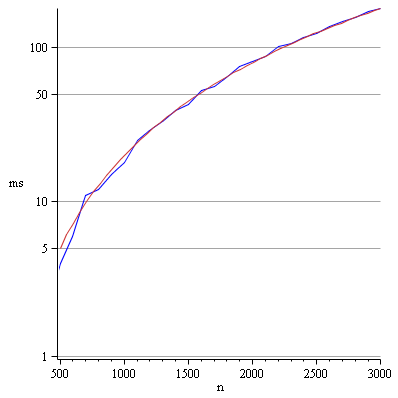
\includegraphics[width=80mm]{RNN_runtime.png}
\caption{The running time of the Reverse Nearest Neighbor algorithm fitted to $x^2$.}
\label{rnn} 
\end{figure}

The blue graph in Figure~\ref{rnn} represents the runtime of our RNN implementation. The orange curve is a fitted $x^2$ function. As expected, the complexity of the algorithm is $O(N^{2})$.

\subsubsection{Global Greedy}

\begin{figure}[ht!]
\centering 
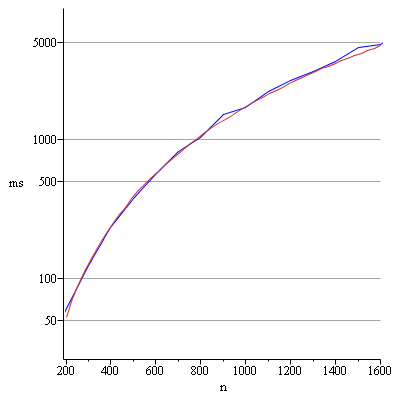
\includegraphics[width=80mm]{GG_runtime.png}
\caption{The running time of the Global Greedy algorithm fitted to $x^2 \cdot log(x)$.}
\label{gg} 
\end{figure}

The blue graph in Figure~\ref{gg} represents the runtime of our GG implementation. The orange curve is a fitted $x^2 \cdot log(x)$ function. As expected, the complexity of the algorithm is $O(N^{2} \cdot log(N))$, which comes from sorting the distances.

\subsubsection{Stable Marriage}

\begin{figure}[ht!]
\centering 
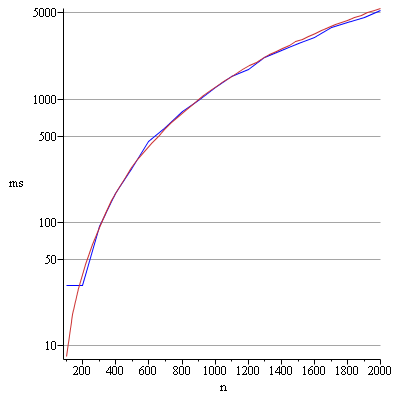
\includegraphics[width=80mm]{SM_runtime.png}
\caption{The running time of the Stable Marriage algorithm fitted to $x^2 \cdot log(x)$.}
\label{sm} 
\end{figure}

The blue graph in Figure~\ref{sm} represents the runtime of our Stable Marriage algorithm implementation. The orange curve is a fitted $x^2 \cdot log(x)$ function. As expected, the complexity of the algorithm is $O(N^{2} \cdot log(N))$, which comes from preparing the input matrix for the algorithm. We have to sort the rows and columns.

  If the distance matrix is $n$ x $m$, then to sort one row takes $m \cdot log(m)$ time. Similarly, to sort one column, it takes $n \cdot log(n)$ time. Therefore, the sorting takes $m \cdot n \cdot log(n) + n \cdot m \cdot log(m)$. Thus, if we denote the maximum of $n$ and $m$ by $N$, the time required for sorting is $O(N^{2} \cdot log(N))$. 

The complexity of the original algorithm was proven to be $N^{2}$. Hence we notice that applying the algorithm to our specific problem increases the complexity. The increase is not very significant though.

\subsubsection{Hungarian Algorithm}

\begin{figure}[ht!]
\centering 
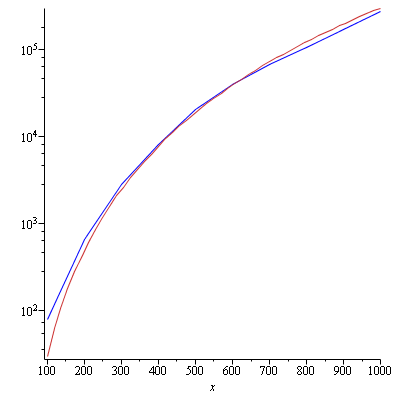
\includegraphics[width=80mm]{HA_runtime.png}
\caption{The running time of the Hungarian Algorithm fitted to $x^4$.}
\label{hung} 
\end{figure}

The blue graph in Figure~\ref{hung} represents the runtime of our HA implementation. The orange curve is a fitted $x^4$ function. As expected, the complexity of the algorithm is $O(n^{4})$. Note that it is possible to implement the Hungarian Algorithm in $O(n^{3})$.

The higher complexity compared to the other matching algorithms is because the Hungarian algorithm aims to assign the objects in such a way that the overall cost of all assignments is minimal, i.e. to find the overall optimal solution.

\subsubsection{Comparison of the Running Times}
The results of the runtime experiment are provided in Table~\ref{runtimes}. Our implementations are not optimal and hence it's hard to compare the absolute values. We still think that the implementations are good enough to allow for some basic deductions.


It is clearly seen that because of its simplicity and the early exclusion of non-unique best matches, the Reverse Nearest Neighbor algorithm is the fastest one. The Global Greedy and the Stable Marriage algorithms are noticeably slower. One of the reasons is that their job differs a bit from the one RNN is doing. GG and SM are making as many matches as possible, even when there are non-unique smallest distances. They both simply pick one of the possible matches. Moreover, GG and SM ensure stable matching which comes with a cost. These two algorithms are comparable because of the stability of their solutions.

The Hungarian Algorithm is by far the slowest, but since it's complexity is much higher we can not really compare it.

In this part we used random double values [0,1] to fill the matrix. We then experimented with different functions that reflect real world data more closely, e.g. $max(0,min(1,log(x*10 + 1)/2))$ (Figure \ref{logfill}), feeding it random double values [0,1]. We noticed that the runtime did not differ much from our previous tests (as we expected). Then we started using functions that resulted in a high amount of lowest values for rows and column. Now all algorithms became faster and the HA was for low $n$ much faster than the SM and GG. This was expected as now there were a lot of optimal solutions available.

\begin{figure}[ht!]
\centering 
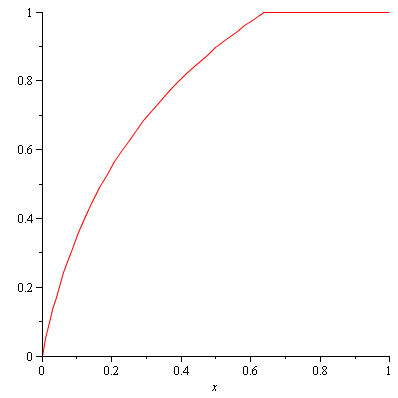
\includegraphics[width=80mm]{logfunction.png}
\caption{$max(0,min(1,log(x \cdot 10 + 1)/2))$ on [0,1]}
\label{logfill} 
\end{figure}

\begin{table}[tbh]
\centering
\begin{tabular}{|c|c|c|c|c|}
\hline 
Size & RNN & Global Greedy & Stable Marriage & Hungarian \tabularnewline
\hline 
\hline 
 100 & 1 & 63 & 20 & 269\tabularnewline
\hline
 200 & 2 & 159 & 40 & 640\tabularnewline
\hline 
 300 & 0 & 90 & 90 & 1826\tabularnewline
\hline 
 400 & 0 & 368 & 190 & 5243\tabularnewline
\hline 
 500 & 2 & 235 & 271 & 11415\tabularnewline
\hline 
 600 & 4 & 276 & 412 & 26197\tabularnewline
\hline 
 700 & 5 & 440 & 600 & 43786\tabularnewline
\hline
 800 & 8 & 961 & 743 & 85837\tabularnewline
\hline 
 900 & 11 & 1269 & 1033 & 135179\tabularnewline
\hline
 1000 & 17 & 1673 & 1265 & 217143\tabularnewline
\hline 
\end{tabular}
\caption{Running times for different sizes.}
\label{runtimes}
\end{table}

\subsection{Quality Tests}

The recall, precision and F-1 measure values of all four algorithms for our different datasets\footnote{The datasets can be found here: \url{http://www.inf.unibz.it/dis/teaching/SS/} (Proposal 6)} are provided in Table~\ref{recall}, Table~\ref{precision} and Table~\ref{fmeasure} respectively. 

The first thing we noticed is that RNN has the highest precision, but a lower recall. This can be explained since it only matches two items if they are the unique best choice for each other. The decision making is not influenced by other matches, resulting in high precision but low recall values (matches are not made if the algorithm is "unsure").

Another interesting observation is that the recall values of GG, SM and Hungarian are very similar in all the cases. Recall values of GG and SM are even equal. % Discuss the reasons

We have shown that GG and SM will produce equal results if the matrix entries are unique. We did not check whether the matchings were identical. Since most non-unique values in the data files were ones, the algorithms might not "reach" them and this could well be the case.

The other noticeable thing is that for all the algorithms except RNN, the recall value is equal to the precision value. Here the explanation lies in the nature of the algorithms: they always make $min(\#rows, \#columns)$ matches. Therefore the number of false positives becomes equal to the number of false negatives in the formulas of precision and recall. And thus, from the definitions of the precision and recall follows, that precision becomes equal to recall.

% Read and say whether you agree. I am not totally sure about it.

\[P = \frac{tp}{tp+fp}, R = \frac{tp}{tp+fn}.\]

\[fp=fn \Rightarrow R=P.\]

\begin{table}[tbh]
\centering
\begin{tabular}{|c|c|c|c|c|}
\hline 
Data File & RNN & Global Greedy & Stable Marriage & Hungarian \tabularnewline
\hline 
\hline 
 Np3q2.dm & 79.26\% & 85.95\% & 85.95\% & 86.29\%\tabularnewline
\hline
 Nw3p2q.dm & 80.27\% & 89.3\% & 89.3\% & 89.97\%\tabularnewline
\hline 
 Nw5p1q.dm & 81.94\% & 92.64\% & 92.64\% & 92.98\%\tabularnewline
\hline 
 Nw8p2q.dm & 82.94\% & 89.97\% & 89.97\% & 89.63\%\tabularnewline
\hline
\end{tabular}
\caption{Recall of different algorithms for different data.}
\label{recall}
\end{table}

\begin{table}[tbh]
\centering
\begin{tabular}{|c|c|c|c|c|}
\hline 
Data File & RNN & Global Greedy & Stable Marriage & Hungarian \tabularnewline
\hline 
\hline 
 Np3q2.dm & 99.16\% & 85.95\% & 85.95\% & 86.29\%\tabularnewline
\hline
 Nw3p2q.dm & 98.77\% & 89.3\% & 89.3\% & 89.97\%\tabularnewline
\hline 
 Nw5p1q.dm & 98.79\% & 92.64\% & 92.64\% & 92.98\%\tabularnewline
\hline 
 Nw8p2q.dm & 98.41\% & 89.97\% & 89.97\% & 89.63\%\tabularnewline
\hline
\end{tabular}
\caption{Precision of different algorithms for different data.}
\label{precision}
\end{table}

\begin{table}[tbh]
\centering
\begin{tabular}{|c|c|c|c|c|}
\hline 
Data File & RNN & Global Greedy & Stable Marriage & Hungarian \tabularnewline
\hline 
\hline 
 Np3q2.dm & 88.1\% & 85.95\% & 85.95\% & 86.29\%\tabularnewline
\hline
 Nw3p2q.dm & 88.56\% & 89.3\% & 89.3\% & 89.97\%\tabularnewline
\hline 
 Nw5p1q.dm & 89.58\% & 92.64\% & 92.64\% & 92.98\%\tabularnewline
\hline 
 Nw8p2q.dm & 90.02\% & 89.97\% & 89.97\% & 89.63\%\tabularnewline
\hline
\end{tabular}
\caption{F-1 measure of different algorithms for different data.}
\label{fmeasure}
\end{table}

\section{Conclusions}

While all algorithms perform a similar task, they are quite different. There are certain features an algorithm can guarantee, but it then pays in complexity. The lowest complexity is acquired by the RRN, which does not guarantee neither stability nor the optimality of the solution. GG and SM have a slightly increased complexity and guarantee the stability of the solution. The most expensive feature is global optimality, which is guaranteed by the Hungarian Algorithm. We notice that an optimal solution is not necessarily a stable one.

In general we can say that the RNN is very good if you want to "be sure" about the matches you make. The other algorithms should be used if you want to make as many matches as possible. Our testing suggests that the quality measures of the HA are slightly better than GG (or SM). However this is not always the case as \textit{Nw8p2q.dm} shows. In most cases the difference will not justify the \textit{much} higher complexity. 

We conclude that neither optimality nor stability is a better property for making the matching. The algorithm you choose should always depend on the data and your preferences. Selecting the correct algorithm is not a trivial task and in certain cases it might be a good idea to hand-match some data and see which algorithm performs best.

\section{Manual}

\textit{Start the program and follow the instructions.}

There are three different modes: "Quality" check, "Runtime" check and "Verify".

When you select the quality check you can load matrices of your choice into the program and all algorithms will run on the data, giving you recall, precision and F-1 measure results. The format for the data should be the same as for the provided test-files (e.g. "Nw8p2q.dm").

The runtime check lets you test the runtime of a selection (or all) of the discussed algorithms. You can select the starting size $n$ of a $n$x$n$ matrix, the step-size by which to increase this $n$ and the amount of steps to perform. Be careful not to choose the amount of steps too high. The matrices are generated using random double values in [0,1].

If you choose to "verify", the program will perform all our implementation checks as discussed in the section "Implementation Testing". As long as you don't change the program, you should not see any errors.

%-----------------------------------------------------------
\addcontentsline{toc}{chapter}{\numberline{}Bibliography}

\begin{thebibliography}{9999}
%\enlargethispage{\baselineskip}
\bibitem{augsten}
Augsten, N.: Approximate Matching of Hierarchical Data. 
Ph.D. Dissertation, Department of Computer Science Faculty of Engineering and Science Aalborg University
\bibitem{gale}
Gale D.; Shapley L. S., College Admissions and the Stability of Marriage, The American Mathematical Monthly,  69(1): 9–15, 1962.

\bibitem{rnn}
Nikolaus Augsten and Michael B?hlen and Johann Gamper: The pq-Gram Distance between Ordered Labeled Trees, Free University of Bozen-Bolzano, 2010 

\bibitem{ha_firstpub}
Munkres, James: Algorithms for the Assignment and Transportation Problems, Journal of the Society for Industrial and Applied Mathematics, 5(1): pp. 32-38, Mar., 1957

\end{thebibliography}

\end{document}
